\chapter{Specification}
\label{Chapter:Specification}

As with every software project, a list of requirements has to be produced in order to define the scope of the software (i.e. what it does) before proceeding to its implementation. That normally involves communication with the client \citep[23]{bell2005}. Due to the lack of a specific client (my audience is a rather group of people), my supervisor agreed on taking part in the requirement gathering process as my client. The specification of the mobile application can be split into three components: Goal-setting, Monitoring and Feedback. The Goal-Setting Component (GSC), as the name implies, handles setting goals as well as providing additional information such as recommended amounts of physical activity per day. The Monitoring Component (MC) is the most complex part of the system. It is essentially a \gls{har} system with additional logic for recognising the current activity of the user (e.g. walking or static) and logging the data into a database. In addition, this component is responsible for detecting sedentary behaviour and measuring physical activity amounts. As far as the Feedback Component (FC) is concerned, it provides feedback to the user in the form of notifications.

\section{Functional Requirements}
    Functional are the requirements that concern the system directly. They state what the software product should do or how it should behave when certain conditions are met \citep[84]{sommerville2010}. During the requirements modelling process a set of use cases was compiled to help with the documentation of the requirements (full list of uses cases can be seen in Appendix \ref{use_cases}). According to \citet[45]{bell2005}, this approach has been used extensively in the past to document functional requirements. Bell also advocates the use of use case diagrams when describing a system's requirements. Thus a use case diagram of the system was developed (see figure \ref{fig:use-case-diagram}).
    
    \begin{figure}
        \centering
        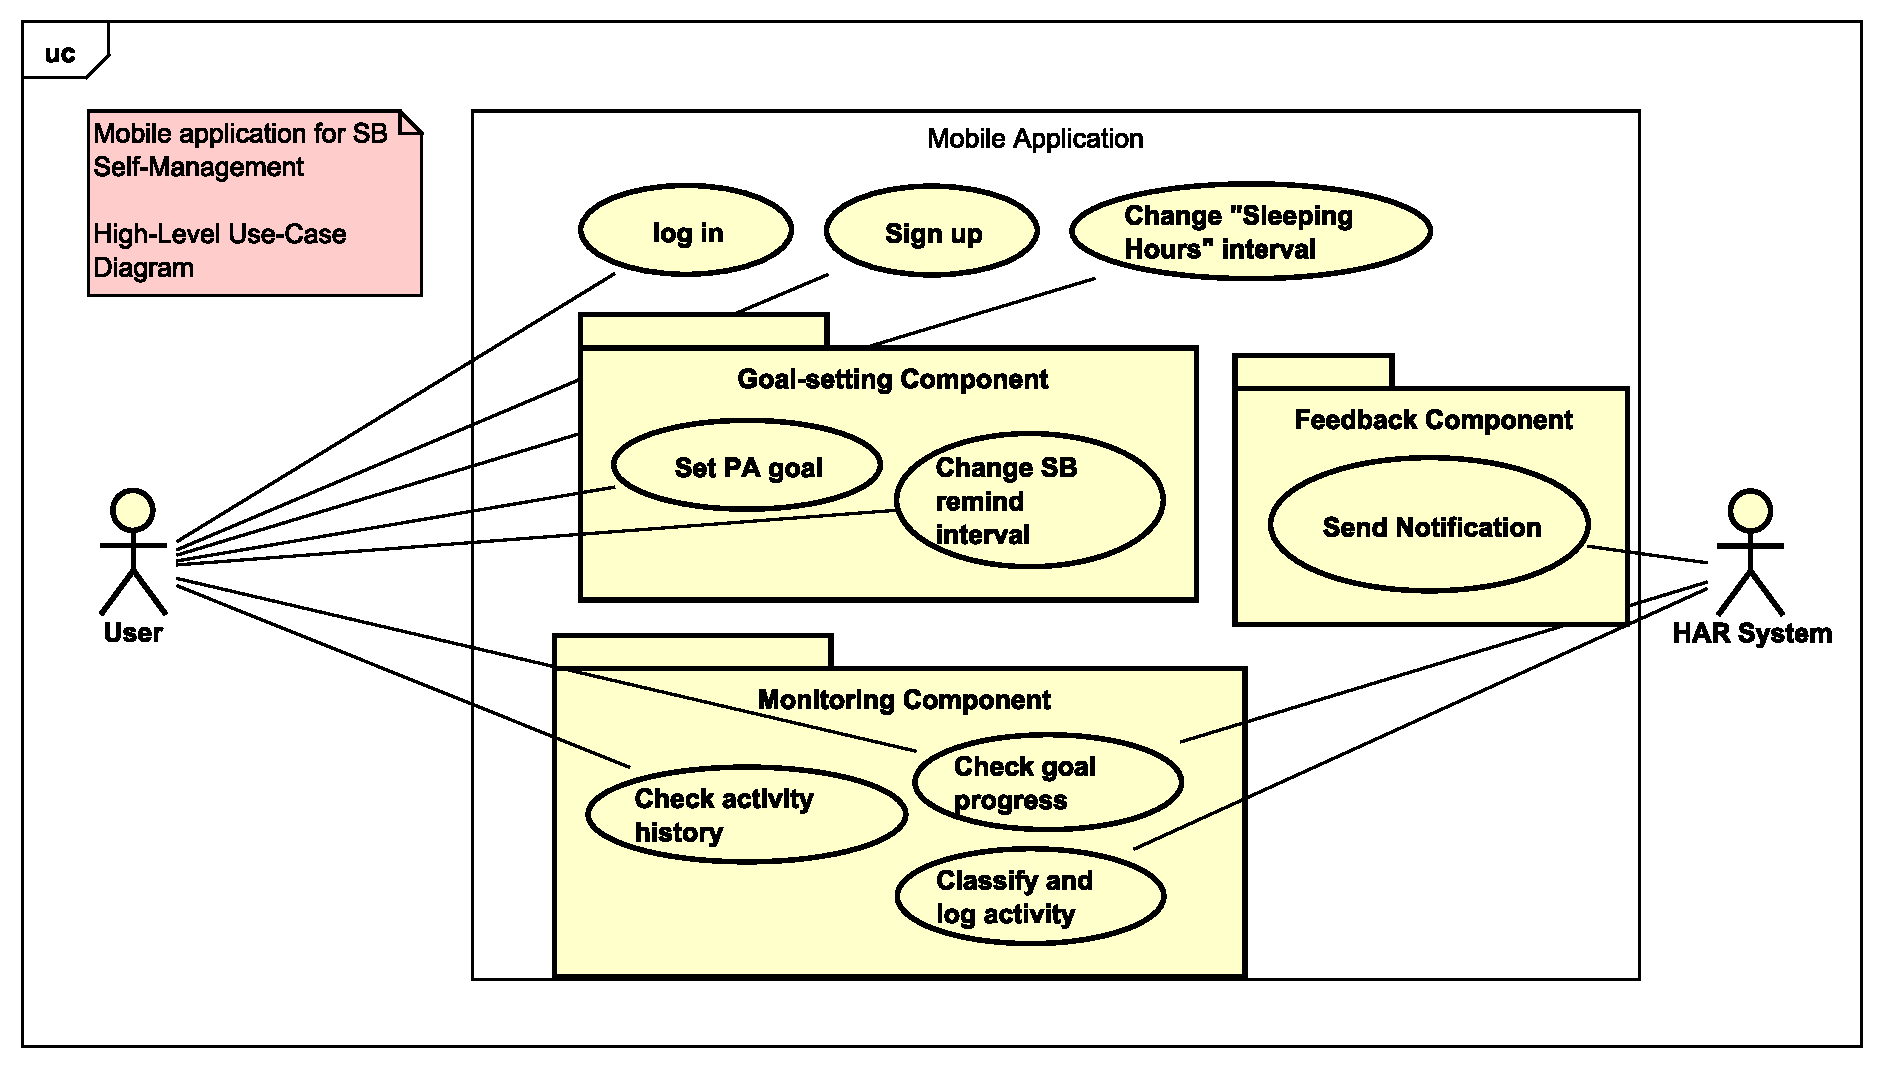
\includegraphics[width=12cm]{use_case_diagram}
        \caption{Use case diagram of \textit{"Active Minutes"}}
        \label{fig:use-case-diagram}
    \end{figure}
    
    \subsection{Goal-Setting Component}
    As it was mentioned in Chapter \ref{Chapter:Literature-Review},  goal-setting is an important part of the behaviour change process. This component's requirements are mainly derived from the background research. Its software implementation would allow the user to set goals which is the first step towards better lifestyle.
    
    \begin{enumerate}
        \item \gls{gsc} shall allow the user to set \gls{pa} goals
        \begin{enumerate}
            \item \gls{gsc} shall provide list of recommended \gls{pa} goals
            \item \gls{gsc} shall allow the user to set custom \gls{pa} goals
        \end{enumerate}
        \item \gls{gsc} shall allow the user to set Sedentary Time (\gls{st}) goals
        \begin{enumerate}
            \item \gls{gsc} shall allow the user to set the maximum duration of \gls{st} before a reminding notification is sent 
        \end{enumerate}
    \end{enumerate}
    
    
    \subsection{Monitoring component}
    The main purpose of the \gls{mc} is to continuously recognise activities and analyse the levels of \gls{pa} and \gls{st}. The following requirements have been derived from analysing past and current mobile devices and applications.
    
    \begin{enumerate}
        \item The \gls{mc} component shall classify physical activities
        \begin{enumerate}
            \item HAR component shall recognise the following activities:
            \begin{enumerate}
                \item walking
                \item running
                \item cycling
                \item static
            \end{enumerate}
        \end{enumerate}
        \item The \gls{mc} component shall analyse user's \gls{pa} and \gls{st} amounts in real time
            \begin{enumerate}
                \item \gls{mc} shall increment user's \gls{pa} or \gls{st} value whenever physical activity or sedentary behaviour is recognised
            \end{enumerate}
        \item The \gls{mc} shall personalise \gls{har}'s classifier
            \begin{enumerate}
                \item When enough user data is collected, the system shall retrain the classifier with user's own data
            \end{enumerate}
            
        \item \gls{mc} shall keep history of previously accumulated \gls{pa} and \gls{st} amounts
        
        \item The user shall be able to set "Sleeping Hours", time interval during which no measurement of \gls{pa} or \gls{st} should occur
      
    \end{enumerate}
    
    \subsection{Feedback Component}
    The \gls{fc} is responsible for sending notifications to the user. It can provide important information such as when a previously set goal is attained or reminder for the user that they are spending too much static time.
    \begin{enumerate}
        \item \gls{fc} shall notify the user when they are being sedentary for too long (e.g. an hour)
        
        \item \gls{fc} shall notify the user when a previously set goal is attained (e.g. being active for 30 minutes)
        
        \item \gls{fc} shall not send notifications during "Sleeping Hours" time interval
    \end{enumerate}

\section{Non-functional Requirements}
The mobile application proposed in this work has to comply with a number of additional requirements. According to \citet[87]{sommerville2010}, Non-functional are those requirements that do not concern the system directly. They apply constrains to the whole system such as performance and security.  Since the \gls{gsc}, \gls{mc} and \gls{fc} are all part of the same software, their non-functional requirements will be discussed all together.
    
    % \subsection{Limitations}
    
    \subsection{Accuracy}
    The accuracy of the system shall be high so that misclassification of activities are avoided or minimised. For example, classifying "walking" as "static" would lead to incorrect \gls{pa} daily readings. Consequently, the user may be doing less physical activity if they are notified they attained a goal.
    
    \subsection{Battery consumption}
    Since the resources of every portable device (i.e. mobile phone) are constrained, the system shall be designed so that it consumes reasonable amount of battery power. For example, the user must not need to charge the device in the middle of the day since that renders measuring component of the application useless (the application cannot measure \gls{pa} when the device is on the user).
    
    \subsection{Security}
    The mobile application shall store user data only on the system in order to minimise the risk of data breach. In addition, the following considerations have been taken into account:
    
    \begin{enumerate}
        \item The system shall provide protection of user's data
            \begin{enumerate}
                \item The system shall show authentication screen before showing any sensitive data
                \item The system shall encrypt the data stored in a local database
            \end{enumerate}
    \end{enumerate}
    
    \subsection{System Quality Attributes}
        
        \subsubsection{Adaptability}
        Modern mobile applications should be able to quickly adapt to new requirements as the market always changes. That is why the system design implements the \gls{mvp} software pattern which increases the ability of the system to incorporate new features easily.
        
        \subsubsection{Scalability}
        It is difficult to envision how much data will be gathered from the sensors of the smartphone. However, the system should be scalable and thus capable of handling large amounts of computations.
        
        \subsubsection{Modularity}
        The system is comprised of different units. For example, each screen is encapsulated in a separate directory which can be interchanged easily without changing the integrity of the system.  
        
        \subsubsection{Testability}
        To assure that the system works as intended, the system shall be tested by both assertions and Quality Assurance tests. 
        
        \subsubsection{Maintainability}
        The system shall be designed in such a way so that it allows for easy debugging and evolution. For example, extending the system by adding new features.
        
        \subsubsection{Robustness}
        The system will constantly work in the background (e.g. collect contextual data) so ensuring that the system encompass as many points of failure as possible is crucial.
    
    
    